\documentclass[]{IEEEtran}
\usepackage[utf8]{inputenc}
\usepackage{algorithm2e}
\usepackage{algorithmic}
\usepackage{amsmath}
\usepackage{amssymb}
\usepackage{caption}
\usepackage{graphicx}
\usepackage{hyperref}
%\usepackage{appendix}

\begin{document}

%opening
\title{Aplicación Movil Para Intercambio de Libros BookSwapp}
\author{Ivan Yesid Castellanos, Osman David Jimenez, Victor Gabriel Ramirez}

\markboth{Desarrollo de aplicaciones para dispositivos móviles, 2017 - III}
{Shell \MakeLowercase{\textit{I. Castellanos, O. Jimenez, V. Ramirez}}: Aplicación Movil Para Intercambio de Libros BookSwapp}

\maketitle

\begin{abstract}
Aqui va el abstract
\end{abstract}

\begin{IEEEkeywords}
	palabras clave
\end{IEEEkeywords}

\IEEEpeerreviewmaketitle

\section{Introducción}

Actualmente el manejo de los libros es bastante desprovechado, dado que una persona necesita un libro por algún tiempo determinado pero despues ya no lo vuelve a utilizar. Un ejemplo muy frecuente es en los textos académicos, los cuales se utilizan en muchos casos solo por un semestre o un año, mientras se ve alguna actividad académica, y despues quedan sin utilizar. Otro ejemplo al respecto son las novelas, las cuales una persona puede leerlas un par de veces y luego ya pierde interés en el texto dado que ya lo leyó.\\
En general, en estos casos, los libres tienen una significativa perdida de valor comercial, por lo que venderlos de segunda no es una buena alternativa, al igual que tampoco lo es conservar los libros que la persona ya no necesite, por esta razón se lantea el proyecto BookSwapp, la cual es una aplicación móvil que permite manejar trueques entre libros de forma sencilla y flexible y así obtener una alternativa para aprovechar los libros que una persona no necesit, cambiandolos por libros que sean de su interés.

\section{BookSwapp}

Ola Ke Ase 

\subsection{Usuario Gratuito}

Esto es una subsección

\section{Resultados}

Aqui poner como resulto todo

\begin{figure}
	\centering
	\captionsetup{justification=centering}
	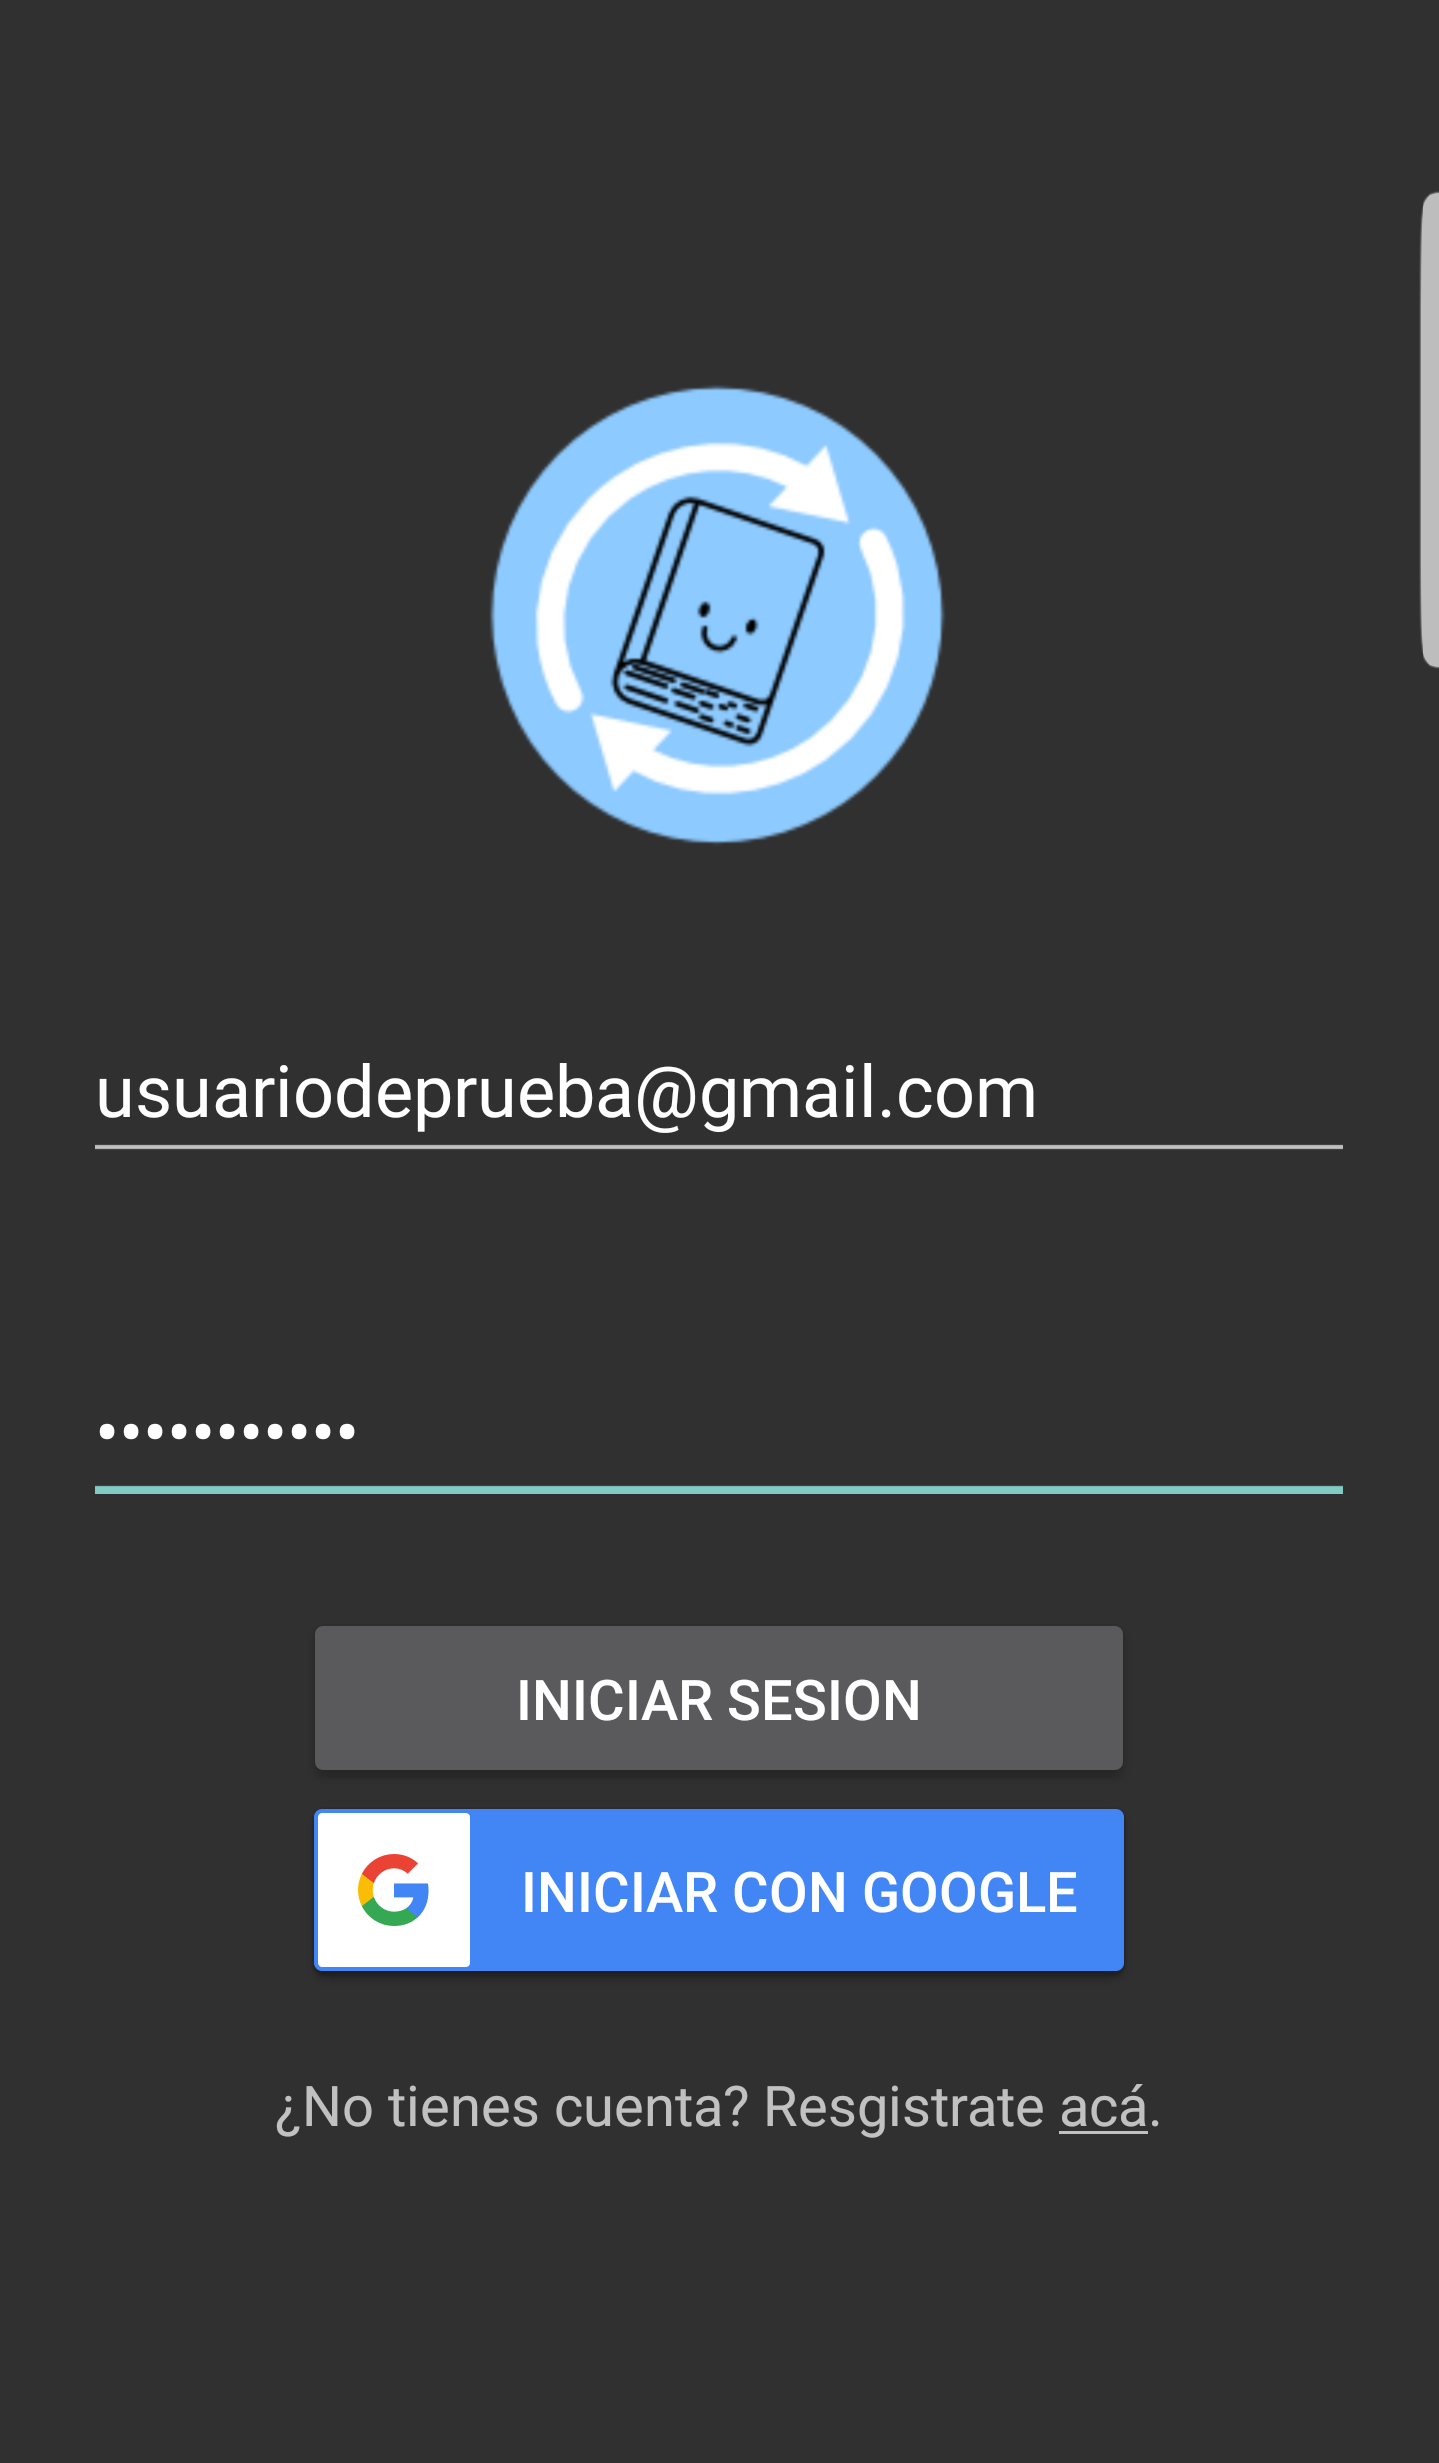
\includegraphics[width=100px]{login.png}
	\hspace{5px}
	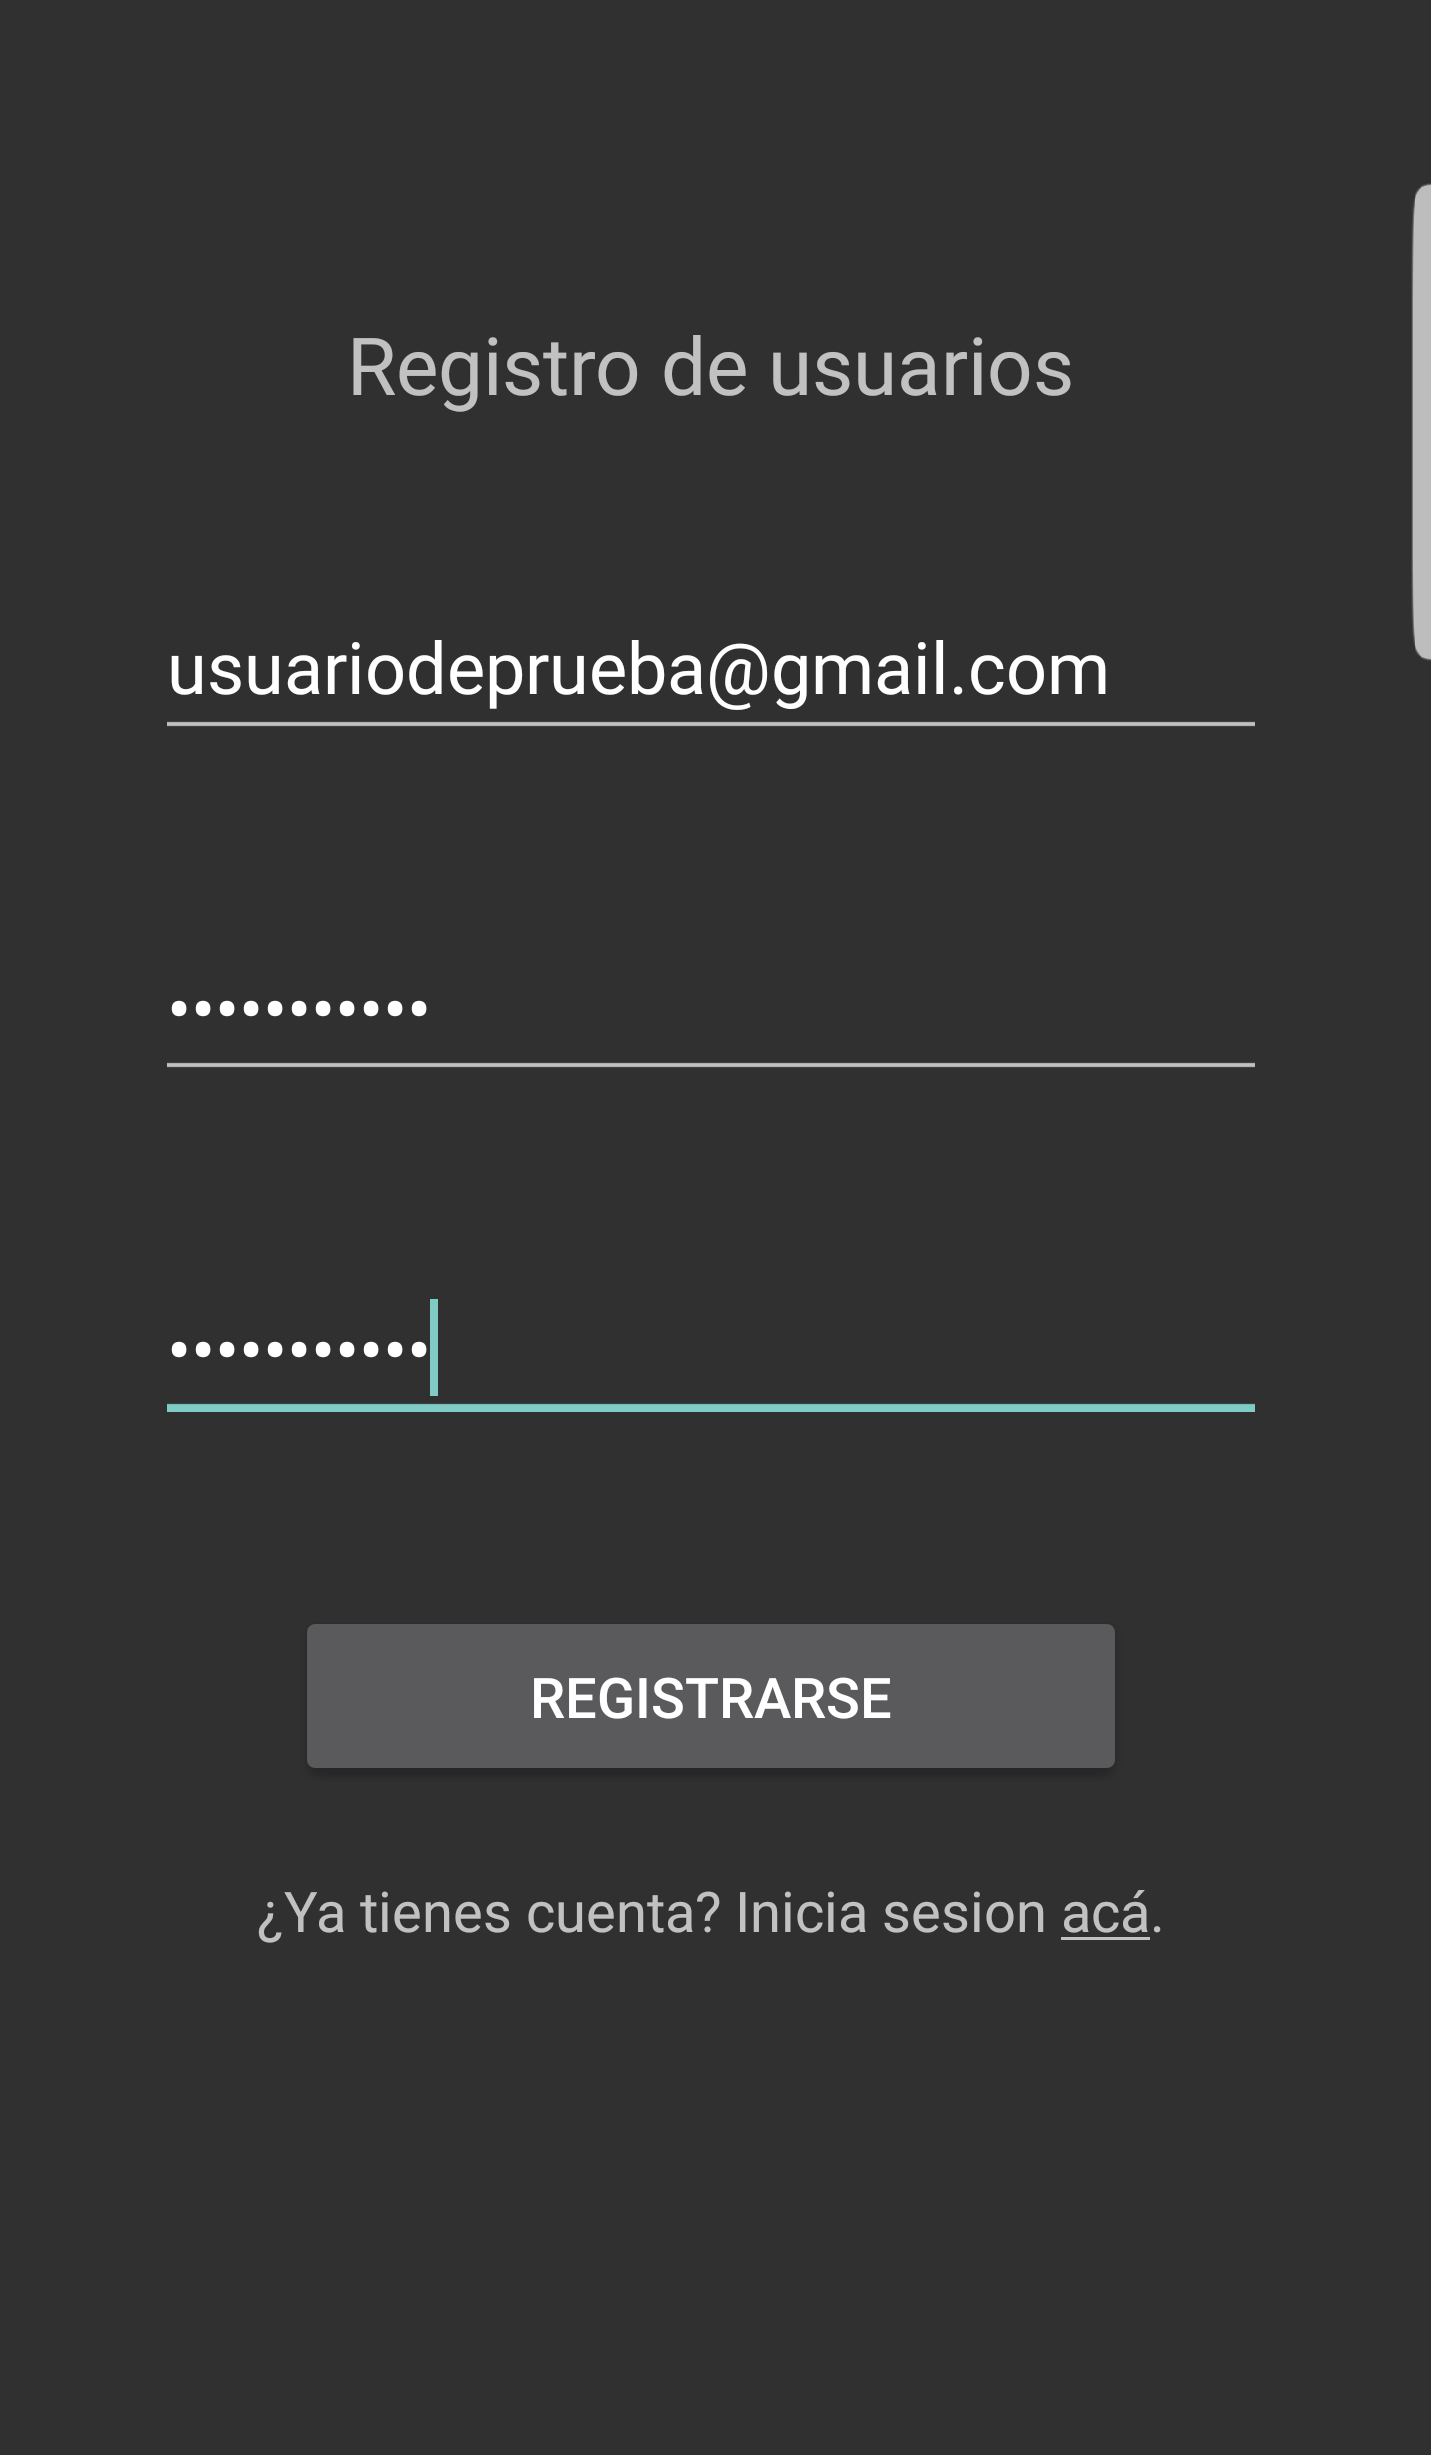
\includegraphics[width=100px]{registro.png}
	\caption{Login y registro}
	\label{FI12}
\end{figure}

\section{Conlusiones}

Conclusiones del trabajo

%\bibliographystyle{IEEEtran}

%\bibliography{bibliografia}

%\newpage

%\section*{Anexos}

%\subsection{Anexo 1. }\label{sec:Anexo1}

%Por si necesitamos anexos

\end{document}
